%\documentclass[nonumbib,leqno]{nrc1}
\documentclass[11pt]{article}
\usepackage{amssymb, amsmath, bm, epsfig,psfrag,graphicx,caption,verbatim,url}
\usepackage[margin=1in]{geometry} %added for white paper 
%commented out for white paper %\usepackage[french, english]{babel}
\usepackage{setspace}
\usepackage{lineno}
\usepackage{natbib}
\usepackage{longtable}
\usepackage{booktabs}
%added 9/29/08
%\usepackage[nolists]{endfloat}

%the following all commented out for white paper
%\bibpunct{(}{)}{;}{a}{}{;}
%\setlength{\mathindent}{1cm}
%\LTcapwidth=\textwidth
%\renewcommand{\tablename}{\textbf TABLE}

%\setcounter{page}{1}
%\volyear{XX}{201X}
%\journal{Can. J. Fish. Aquat. Sci.}

%\received{}

\bibliographystyle{ecology}

\begin{document}

%the following all commented out for white paper
%\title{Use and misuse of survey data to detect prey removal effects on Steller sea lions ({\it Eumetopias jubatus})}

%\author[P. B. Conn, D. S. Johnson, L. W. Fritz, B. S. Fadely]{Paul B. Conn, Devin S. Johnson, Lowell W. Fritz, Brian S. %Fadely}
%\address{National Marine Mammal Laboratory, Alaska Fisheries Science Center,
%NOAA National Marine Fisheries Service,
%Seattle, Washington, U.S.A. 98115}
%\correspond{paul.conn@noaa.gov}

%\shortauthor{Conn et al.}
%\large
%maketitle
%{\sc Running Head}: Prey removal and Steller sea lions \bigskip

%the following added for white paper
\begin{center}
{\bf Use and misuse of fishery and survey data to detect prey removal effects on Steller sea lions ({\it Eumetopias jubatus})}

\bigskip

\vspace{3in}

Paul B. Conn \footnote[1]{email:paul.conn@noaa.gov}, Devin S. Johnson, Lowell W. Fritz, Brian S. Fadely

\vspace{0.5in}

National Marine Mammal Laboratory, Alaska Fisheries Science Center,
NOAA National Marine Fisheries Service,
Seattle, Washington, U.S.A. 98115 \\

\vspace{1in}


Sep 11, 2013
\end{center}


\clearpage

%commented out for white paper \linenumbers

%% ABSTRACT %%%%%%%%%%%%%%%%%%%%%%%%%%%%%%%%%%%%%%%%%%%%%%%%%%%%%

%{\sc Summary.}

% commented out for white paper   \begin{abstract}
{\bf ABSTRACT} %added for white paper
\large
Surveys of Steller sea lions in the Gulf of Alaska and Aleutian Islands indicated a declining population through 2000, and the western stock of Steller sea lion was listed as endangered under the U.S. Endangered Species Act in 1997.  One focus of mitigation has been to limit fishing activities around Steller sea lion rookeries because of concern that Steller sea lion population dynamics depend in part upon the availability of harvested fish stocks. A
number of studies have attempted to determine the nature of the relationship between fishing and Steller sea lions by fitting statistical models relating Steller sea lion aerial survey metrics (e.g., counts, changes in counts) to fish or fishing variables (e.g., relative abundance, catch, fishing effort), with many tests resulting in an insignificant effect of fishing.  These results, combined with parametric power analyses, recently led a team of independent experts \citep[e.g.,][]{Bernard:2011dq} to conclude that fishing is unlikely to affect Steller sea lion populations.  In this study, we conduct a more comprehensive form of power analysis where we fit a battery of statistical models to data that were simulated from hypothetical populations of Steller sea lions and fish, where sea lion survival or fecundity was explicitly written as a function of fish biomass.  We calibrated predator-prey dynamics such that fishing led to large declines in Steller sea lion populations, and then assessed whether we could detect an underlying relationship between sea lions and fish using typical survey variables.  Our analysis revealed that even under idealized study conditions (independent populations, annual sampling, a single prey species, and an unbiased fish index), that many combinations of dependent and independent variables resulted in poor power or misleading results.  For example, analyses that used fishing metrics (catch, effort) as dependent variables often led to insignificant or positive regression coefficients.  Analyses using adult survey counts as the dependent variable also performed poorly.  We found that analyses conducted with proportional changes in adult counts ($\lambda$) as the dependent variable and fish relative abundance as the dependent variable had high power to detect a relationship between sea lion survival and fish availability. Likewise, analyses relating annual sea lion pup counts to fish relative abundance had the highest power to detect a relationship between sea lion fecundity and fish availability. However, given the idealized study design, our estimates of power are undoubtedly overestimated.  Our results suggest that certain types of analyses (i.e., those using catch or fishing effort as an independent variable or adult counts as a dependent variable) should be avoided entirely, and that results of previous studies using these variables are largely uninformative regarding the effect of prey depletion on Steller sea lion populations.  Further, given a lack of analyses relating pup counts to fish relative abundance in the literature, we find that there is currently little to no information with which to judge whether prey availability affects sea lion fecundity. Future work should be devoted to relating sea lion fecundity to fish relative abundance, and in conducting more detailed simulation tests of power that include more realistic dynamics (e.g., sea lion movement between colonies, spatial autocorrelation).  We describe how results of simulation analyses can be used to help calculate Bayes factors that encapsulate belief about various working hypotheses.
%\keywords{Steller sea lions, }
%commented out for white paper \end{abstract}

%\begin{resume}
%\end{resume}

% commented out for white paper \keywords{Bayes factor, {\it Eumetopias jubatus}, power analysis, predator-prey model, simulation study, Steller sea lions}


\clearpage

\renewcommand{\baselinestretch}{1.8}\normalsize


\section{Introduction}

In 1990, the Steller sea lion (SSL; {\it Eumetopias jubatus}), the largest of the otariid pinnipeds and a prodigious piscivore, was listed as a `threatened' species range-wide under the US Endangered Species Act (ESA) by the US National Marine Fisheries Service (NMFS) after more than a decade-long, 80\% decline in abundance \citep{CalkinsPitcher1982,LoughlinEtAl1992,NMFS1992}.  This sparked a scientific, legal, and management debate about the cause of the decline, and specifically the role of fishery competition \citep{Alverson1992,NMFS1992,FritzEtAl1995,RosenTrites2000,McBeath2004}.  The debate intensified after 2000 as the Steller sea lion's western distinct population segment\footnote[1]{Breeds on rookeries between $144^\circ$W and $140^\circ$E in Prince William Sound through the Aleutian Islands, Commander Islands, Bering Sea, Kuril Islands and Sea of Okhotsk.}  (DPS; recognized in 1997 when it was up-listed to  `endangered' and split from the eastern DPS\footnote[2]{Breeds on rookeries east of $144^\circ$W in southeast Alaska, British Columbia, Washington, Oregon and California.} ) has begun to slowly, but unevenly recover across its range \citep{Loughlin1997,JohnsonFritzInReview, NMFS2013}.  Some of the most common species in the diets of western Steller sea lions are groundfish species \citep[e.g., walleye pollock {\it Theragra chalcogramma}, Pacific cod {\it Gadus macrocephalus}, and Atka mackerel {\it Pleurogrammus monopterygius};][]{ SinclairZeppelin2002,TollitEtAl2004,ZeppelinEtAl2004,McKenzieWynne2008,WaiteEtAl2012} that are also targets of some of the largest and most efficient commercial fisheries in the world \citep{FissellEtAl2013}.

Almost a dozen threats to the western SSL stock have been evaluated as possible proximate or ultimate causes of the original decline and slow, regionally variable recovery since the original ESA listing \citep{FerreroFritz2002,NMFS2008,AtkinsonEtAl2008}.  Some direct causes of mortality that contributed to the steep decline observed in the 1980s were reduced in the 1990s by changes in fishing methods (incidental catch in fishing gear) or regulations \citep[prohibiting shooting at or near a Steller sea lion and 3 nm no-entry zones around sea lion breeding locations;][]{FritzEtAl1995,FerreroFritz2002,NMFS2008}, which likely contributed to the slower rate of population decline observed following the ESA listing.  Other factors (disturbance on terrestrial sites or at-sea, research-related mortality, disease, entanglement in marine debris, and subsistence hunting) are thought or known to occur at levels too low to threaten recovery \citep{AtkinsonEtAl2008,NMFS2008}.  New information on mercury in SSL in the Aleutians Islands has raised concerns about the impact that contaminants may play in the continued declines observed in this area \citep{CastelliniEtAl2012,ReaEtAl2013}, but while total mercury concentrations in some newborn pups from the western Aleutian Islands were at levels that are associated with deleterious neurological and reproductive effects in other fish-eating mammals \citep{ReaEtAl2013}, there is no apparent correlation between mean mercury concentration and recent trends in pup production on a regional basis \citep{CastelliniEtAl2012}; more research on mercury in sea lions is necessary to fully evaluate its impact on recovery.  Predation by mammal-eating [transient, Bigg's] killer whales ({\it Orcinus orca}) is certainly a major cause of mortality, particularly for young sea lions \citep{HeiseEtAl2003,SpringerEtAl2003,WilliamsEtAl2004,ManiscalcoEtAl2007,HorningMellish2012}, but may not be a significant threat to recovery considering that population densities of transient killer whales are unrelated to regional western SSL population trends \citep{ZerbiniEtAl2007,DurbanEtAl2010,JohnsonFritzInReview}.  The most problematic of the potential threats is nutritional stress related to decreased availability or quality of prey, and the problem arises because the two possible sources, natural or anthropogenic (fisheries competition), manifest identically in sea lions yet would necessitate vastly different management responses if it were known which was primarily responsible for observed sea lion trends.  `Natural' nutritional stress has been hypothesized to be related to oceanographic cycles (decadal 'regime' shifts) that alternately favor recruitment of high (e.g., Pacific herring {\it Clupea pallasii}) and low energy species (e.g., gadids such as walleye pollock and Pacific cod; \citealt{MantuaEtAl1997,HuntStabeno2002,TritesEtAl2007}, but also see \citealt{RudnickDavis2003,FritzHinckley2005}).  When low energy species are abundant, there would be little that management could do to assist in the recovery of Steller sea lions if their populations declined.  Fisheries may also reduce the availability of prey to Steller sea lions at local, meso- or ecosystem scales to such an extent that population trends (e.g. survival and birth rates) are affected \citep{NMFS2003,NMFS2008}.   Section 7 of the ESA requires NMFS to ensure that federal actions (e.g., authorization of US groundfish fisheries off Alaska) do not jeopardize the continued existence or adversely modify critical habitat of listed species; knowledge of the relative magnitude of natural and anthropogenic factors in inducing nutritional stress would be helpful for this process.

Unfortunately, experiments that directly test for effects of commercial fisheries on SSL population dynamics through a prey availability mechanism have not been conducted due to logistic difficulties and prohibitive costs associated with the large-scale and long-term study design that would be required \citep{FerreroFritz2002}, as well as with constructing a study to meaningfully deplete the prey base of an endangered species legally under the ESA \citep{Bryant2009}. In the absence of such experiments, a series of published and unpublished studies have instead attempted to statistically test the hypothesis that SSL abundance or changes in population trajectory can be explained by commercial fishery activity \citep{Loughlin:1989kl,Ferrero:1994hc,Sampson:1995cr,Dillingham:2006fv,Hennen:2006bs,Soboleff:2006fk,Calkins:2008ve,afsc:2010dz,
Trites:2010ly,Hui:2011uq}. Most of the studies utilize a similar approach, characterized by either correlative analysis or fitting linear or curvilinear models to sea lion count data and some metric of fish abundance, fishery effort, or fishery catch as a predictive covariate. Among all the statistical tests of the ten studies cited above, most (89\%) resulted in statistically non-significant associations, with relatively few that are significantly positive (6\%) or negative (5\%). For fishery variables (effort or catch), statistically significant negative regression coefficients have often been interpreted as ``negative" effects of fisheries activity on SSL abundance, while statistically positive associations and non-significant results are often interpreted as indicating fishing removals had no effect on sea lion populations (note that the interpretation of positive and negative effects are reversed when a fish abundance proxy is used as a predictor). However, the overwhelming number of non-significant relationships calls into question the appropriateness of the underlying models and data treatments, and also whether findings of significant effects (positive or negative) are spurious. A lack of consistent model results creates difficulties for fishery and wildlife managers attempting to choose appropriate fishery management measures designed to alleviate potential resource competition. In the fishery management arena, results of unpublished reports and published papers have often been presented with equivalent weights as evidence \citep[e.g., see][]{Bernard:2011dq} regardless of cautions or caveats stated within the studies themselves.

A fundamental issue when testing the prey availability hypothesis (i.e., the hypothesis that SSL vital rates depend on abundance of commercially harvested fish stocks) is the selection of appropriate dependent and independent variables for statistical analysis.  Ideally, such variables would be selected in a manner such that model results could help improve our mechanistic understanding of how changes in prey availability affect Stellar sea lion vital rates \citep{FayPunt2006,Wolf:2008qf}. However, it is unclear which, if any, mechanistic hypothesis each of the studies cited above are testing.  Most of these studies use adult SSL counts to compare directly with measures of fishing effort or prey availability, ostensibly testing the hypothesis that prey availability or fishing effort is related to adult survival. \citet{Loughlin:1989kl} and \citet{Ferrero:1994hc} also consider pup abundance as a variable, both directly and with fishing activity lagged by 1-5 years, ostensibly addressing the hypothesis that prey removal may act on the survival of younger age classes and/or natality.

Sea lion abundance data, fishery effort, and fish abundance data are collected through separate efforts within NMFS or the Alaska Department of Fish and Game (for fishery landings in State waters), and collection of those data occur on different spatial and temporal scales. The studies statistically comparing sea lion and fishery data also vary in how those data were handled, undoubtedly contributing to inconsistent results among studies. Steller sea lion abundance is determined through counts obtained at rookeries and haulouts during the June-July breeding season from aerial or land-based surveys \citep{FritzEtAl2013}. Sea lions are split into two age classes, based on the time of year, as pups ($<2$ months old) and non-pups ($>12$ months old). Depending on the study, as few as 8 sites \citep{Loughlin:1989kl} to as many as 154 sites \citep[though combined into 10 sub-areas;][]{afsc:2010dz} are used to represent abundance for the wDPS range (or portions therein) of SSL in Alaska. Counts are uncorrected for non-pups that may have been at sea during the survey. For comparison with fisheries data, sea lion counts have been used directly \citep{Ferrero:1994hc,Sampson:1995cr,Soboleff:2006fk,Trites:2010ly} or converted into population trends or instantaneous or annual growth rates over specified time periods \citep{Loughlin:1989kl,Sampson:1995cr,Hennen:2006bs,Dillingham:2006fv,Calkins:2008ve,afsc:2010dz,Trites:2010ly,Hui:2011uq} and studies varied in how rookeries and haulouts were geographically clustered for analysis. All studies used some measure of total annual catch, and one or several other metrics of fishing activity estimated from NMFS Fisheries Observer Program data (available online at \url{http://www.afsc.noaa.gov/FMA/fma_database.htm}), though \citet{Trites:2010ly} obtained the same data for the Aleutian Island Atka mackerel fishery from the fishing industry) or State of Alaska Department of Fish and Game landings database \citep{Soboleff:2006fk}. Studies also varied in how fishery metrics were estimated, and how they were spatially and temporally aggregated. Because observer coverage varies with vessel size there is incomplete observer coverage among the commercial fishery fleet; different methods were used to expand observer data to the entire fleet ranging from none at all \citep{Hui:2011uq}, to simple multiplication by expansion factors \citep[e.g.,][]{Dillingham:2006fv,Hennen:2006bs,Calkins:2008ve}, and more sophisticated catch-area-gear blending \citep{afsc:2010dz}. Because the smallest vessels are not required to carry observers, and others have only 30\% coverage, observer data under-represents smaller vessels that typically fish nearer to shore than larger vessels \citep{afsc:2010dz}. All studies used estimates of the total biomass of fish caught for the commercial species of interest in a calendar year within some specified distance or distances of sea lion rookeries and haulouts. Studies also used average fish weight \citep{Loughlin:1989kl}; effort, measured as the time gear was fished or deployed \citep{Sampson:1995cr,Hennen:2006bs,Dillingham:2006fv,Calkins:2008ve}, or as number of gear hauls \citep{Hennen:2006bs,Calkins:2008ve,Trites:2010ly} or number of vessels fishing \citep{Soboleff:2006fk}; catch-per-unit-effort (CPUE) calculated as the sum of catch divided by sum of hours fished \citep{Loughlin:1989kl,Hennen:2006bs,Calkins:2008ve} or as the average catch per haul \citep{Trites:2010ly}; and harvest rate, calculated as the ratio of fish catch to estimated available biomass (derived from NMFS stock assessment surveys, available online at \url{http://www.afsc.noaa.gov/RACE/groundfish/survey_data/default.htm}) or presumed standing biomass calculated by subtracting fishery catch from estimated available biomass \citep{Hui:2011uq}.

In the majority of these studies, fisheries-reported data were used to represent both prey availability and fisheries removals (though not necessarily in an explicit manner). However, fisheries do not randomly target fish biomass, but rather seek aggregations to maximize economic gain; thus fish removals and some measures of effort will be correlated with prey density and the treatment variable is not randomly allocated for testing a prey depletion hypothesis. Catch-per-unit-effort may be an improvement, though how well this metric correlates with standing biomass is a concern. Depending on the fishery, CPUE may not scale linearly with true fish relative abundance or density if nets are only deployed when there is a reasonable certainty of catching the targeted fish \citep{Hilborn1992,SalthaugAanes2003}, or if there are functional constraints to processing catch \citep{Trites:2010ly}. For studies that incorporate standing biomass of fish stocks, NMFS stock-assessment surveys are stratified to generate less-biased estimates of biomass, but the temporal and spatial scale of those estimates may be too course for this type of analysis.

In this paper, we use simulation to investigate whether available SSL aerial survey metrics (adult or pup counts, count ratios) and explanatory variables commonly compiled from fisheries datasets are sufficient to reveal relationships between SSL population dynamics and prey availability. To conduct simulations, we consider the joint dynamics of SSL, a prey population, and a fishery.  A tacit assumption in all of our simulations is that sea lion dynamics depend on availability of the prey resource through one or more demographic component (e.g. fecundity, survival).  Due to data limitations and the complexity of simulated dynamics, our approach makes a number of simplifying assumptions (e.g. spatially independent populations, a single prey species).  However, these simplifications all serve to increase the power of detecting a relationship between fishing and SSL abundance; if statistical power is poor with simulated data, it will be even worse in the real world.

The remainder of this article is structured as follows.  First, we describe a number of alternative models for the coupled fishery and SSL dynamics.  These models are intended to encompass a number of
alternative states of nature, including the functional relationship between sea lions and fish, as well as
how fishing effort is allocated (i.e., whether or not it is dependent on fish distribution).  Next, we provide details on how we calibrated these models to generate reasonable parameter estimates for simulation.  We then describe our overall simulation structure and provide details on the simulation outputs (e.g., conventional test statistics, Bayesian model weights) that we used to measure our ability to detect relationships between SSL abundance and explanatory fisheries variables.  After describing results, we conclude by offering some final thoughts about how best to interpret SSL-fisheries interactions on the base of available data.


\section{Methods}

We considered models for coupled dynamics between fishers, fish, and SSL, where fish and SSL were modeled as island populations (i.e. assuming independent dynamics among islands).  In reality, there is substantial dispersal of SSL among rookery and haulout areas.  Similarly, relevant fish populations in the Gulf of Alaska and Bering Sea (e.g., Atka mackerel, Pacific cod, walleye pollock) are interconnected through movement and recruitment processes.  However, the assumption of independent dynamics should provide greater power for detecting meaningful relationships between SSL aerial survey counts and fishery variables, since responses of SSL to experimental treatments (fishing) are not blurred by uncontrollable and poorly understood processes.  Thus, a simulation design assuming island populations should provide a useful one-way test for whether the approach of relating fishery variables to SSL counts provides reasonable inferences.

\subsection{Models}


To induce coupled dynamics between SSL, fish, and fishers, we modeled
fish mortality as a function of both fishing effort and SSL predation, where annual fish recruitment follows a Beverton-Holt spawner-recruit function \citep{Beverton1957} with lognormal error (separate models for state dynamics are modeled for each island population).  In turn, we made SSL dynamics dependent on the expected per capita number of fish ``harvested" by SSL, where dependency can be expressed in terms of survival or fecundity (depending upon simulation configuration).  Finally, we considered two scenarios for fisher dynamics, allowing fishing effort to be (i) randomly allocated each year, or (ii) allocated in proportion to fish biomass in each island population.  These components are described in further detail below.


\subsubsection{Steller sea lion model}

We based SSL dynamics loosely on the age-structured, (`HFYS') Leslie-matrix model described by \citet{HolmesEtAl2007}, who summarized fecundity and survival probability for SSL for ages $0-30$ (survival probability was assumed zero after age 30).  This model assumes a post-breeding census, coinciding with annual aerial surveys of rookeries and haul-outs in the Gulf of Alaska and Aleutian islands in June and July.  As presented, this `base' Leslie-matrix has a dominant eigenvalue of 1.000, which is indicative of a stable population (at least in absence of demographic stochasticity).

To make SSL demography dependent on the number of fish, we allowed either female fecundity at age ($f_{a,t,k}$) or female survival at age ($S_{a,t,k}$) (Table \ref{tab:model}) to be dependent on the ratio of fish to sea lion biomass.  Survival probability is naturally bounded in the $(0,1)$ interval, while
fecundity is biologically constrained to be in the $(0,1)$ interval (females usually produce a maximum of one pup per year), so we model both parameters on the logit scale:
\begin{linenomath}
\begin{equation*}
{\rm logit}(S^f_{a,t,k})=\alpha_{0,a} + \alpha_1 B_{t,k}^*/X_{t,k} \hspace{2mm} {\rm or}
\end{equation*}
\end{linenomath}
\begin{linenomath}
\begin{equation*}
{\rm logit}(f_{a,t,k})=\beta_{0,a} + \beta_1 B_{t,k}^*/X_{t,k}.
\end{equation*}
\end{linenomath}
Here, $S^f_{a,t,k}$ gives survival of female age $a$ SSL in year $t$ of simulation for site $k$, $f_{a,t,k}$ gives SSL fecundity for age $a$ in year $t$ and site $k$, $B_{t,k}^*$ gives SSL biomass in year $t$ in site $k$, and $X_{t,k}$ gives fish biomass that is exploitable by SSL in year $t$ and site $k$ (for a complete list of notation, see Table \ref{tab:model}).  We modeled male SSL dynamics by assuming a 50/50 sex ratio at age 0, and a fixed ratio $r_a$ between female and male survival thereon (i.e., $S^m_{a,t,k}=r_a S^f_{a,t,k}$).  We calculated $r_a$ using the ratio of male to female survival estimates in \citet{CalkinsPitcher1982}. Biomass of both sexes was calculated using the fitted Richards growth curves provided in Table 2 of \citet{WinshipEtAl2001}. We calibrate parameters describing the hypothetical relationship between demographic parameters and relative biomass of SSL and prey at the start of year $t$ ($\alpha_0,\alpha_1,\beta_0,\beta_1$) in a later section (see \ref{section:Calibration}).

\subsubsection{Prey (fish) model}

A variety of commercially important fish stocks are affected by time-area closures designed to protect SSL, most notably walleye pollock ({\it Theragra chalcogramma}), Pacific cod ({\it Gadus macrocephalus}), and Atka mackerel ({\it Pleurogrammus monopterygius}).  Rather than base fish dynamics on just one (or multiple) of these species, we modeled fish dynamics of a hypothetical, generic species that combined similar life history and exploitation features from each stock.  For simplicity, we use the same annual time step for the fish population as for SSL, modeling recruitment as occurring immediately prior to annual aerial surveys.  An age-structured population dynamics model was assumed for each simulated fish stock, with 10 ages (1-9 and 10+).
We write total mortality rate for a given fish age class $a$ at time $t$ at site $k$ as $Z_{a,t,k}=M + F_{t,k}^* + F_{a,t,k}$, where $M$ gives
natural mortality, $F_{t,k}^*$ gives a mortality rate attributable to SSL in site $k$ in year $t$ of simulation, and $F_{a,t,k}$ gives time- and age-specific fishing morality (recall that notation is also defined in Table \ref{tab:model}).  Recent assessments of walleye pollock, pacific cod, and Atka mackerel stocks \citep[e.g.][]{PollockAssessment2011,PacCodAssessment2011,AtkaAssessment2012} indicated natural mortality rates in the 0.3-0.34 range.  However, these figures include all natural mortality, including SSL predation (which we model separately).  For our hypothetical fish stock, we set $M=0.2$ during simulations.

We modeled fishing mortality, $F_{a,t,k}$, as a product of an age-specific selectivity curve and a fully selected fishing mortality rate that is itself a function of fishing effort, such that $F_{a,t,k}=q E_{t,k} s_a$, where $E_{t,k}$ summarizes fishing effort for site $k$ in year $t$, $s_a$ describes selectivity at age, and $q$ is a catchability coefficient. Note that this formulation assumes a constant and linear relationship between effort and fishing mortality.  Recent assessments of fish stocks in the Bering Sea used flexible selectivity functions that were allowed to evolve over time; these pointed to dome-shaped selectivity functions in the majority of cases.  For simulations, we used a dome-shaped double logistic model constructed so as to approximate the general shape obtained in the assessments (Fig. \ref{fig:at_age}, Table \ref{tab:model}).  For further description of effort and catchability, we refer the reader to subsequent sections \ref{section:Fleet} and \ref{section:Calibration}, respectively.

For SSL-related mortality, we imposed a model of the form $F_{a,t,k}^*=\delta s_a^* N_{t,k} B_{t,k}^*$, where $s_a^*$ gives the relative selectivity of SSL on age $a$ fish, $N_{t,k}$ gives the total number of fish in population $k$ at time $t$, $B_{t,k}^*$ gives the SSL biomass at time $t$, and $\delta$ gives a capture efficiency parameter. This is a similar functional form as used in classic Lotka-Volterra predator-prey models \citep[see e.g.][]{Gotelli2001}, with the modification that we use biomass (instead of numbers) of SSL to allow for the fact that larger sea lions will likely consume more fish than smaller ones.  Once again, we leave it until a later section (\ref{section:Calibration}) to determine reasonable values for $\delta$.

\citet{ZeppelinEtAl2004} reported substantial overlap between sizes of walleye pollock and Atka mackerel harvested by SSL and commercial trawl fisheries, although the distribution of fish lengths selected by SSL was shifted to the left (i.e., towards smaller-sized fish).  SSL selectivity likely varies by a number of factors, including year, SSL size/age, fish availability, and location \citep{ZeppelinEtAl2004}.  For our simulation study, we constructed a double logistic selectivity that was offset from fishery selectivity to have a modal age that was two years less (Fig. \ref{fig:at_age}, Table \ref{tab:model}).

Annual recruitment at each site was modeled using a Beverton-Holt spawner-recruit curve subject to lognormal error.  A popular parameterization of this model is
\begin{linenomath}
\begin{equation*}
N_{1,t+1,k} = \frac{0.8 R_{0,k} h SSB_{a,t,k}}{0.2 \phi_0 R_{0,k}(1-h)+(h-0.2)SSB_{t,k}} \exp{\epsilon_{t,k}},
\end{equation*}
\end{linenomath}
where $N_{1,t,k}$ gives the number of recruits (age 1 individuals) in year $t$ at site $k$, $R_{0,k}$ is expected annual recruitment in absence of fishing (allowed to be different across sites), $SSB_{t,k}$ gives spawning biomass in year $t$, $h$ is steepness, $\phi_0$ is unfished spawning biomass per recruit (calculated in absence of SSL), and $\epsilon_{t,k}$ represents Gaussian noise \citep{Mace1988}.  Spawning stock biomass can be calculated from knowledge of numbers of fish in each age class, together with maturity at age and weight at age vectors (Table \ref{tab:model}).

\subsubsection{Fleet dynamics}
\label{section:Fleet}

We considered two scenarios for fleet dynamics, both of which assume that total fishing effort stays constant
over the course of simulation time (at least in portions of simulation time series where fishing occurs).  In the first scenario, we allow fishing effort to be annually redistributed according to a ${\rm Dirichlet}(1,1,\hdots,1)$ distribution.  This formulation approximates the situation where experimental treatments (fishing) are applied randomly to experimental units (sites).  As such it is clearly unrealistic, as fishing vessels will likely try to optimize catch by going to areas where there are more fish, perhaps subject
to economic and time constraints (e.g., distances from port).  Nevertheless, this scenario likely provides the greatest power to detect relationships between SSL survey counts and fishing variables.

Our second scenario assumes that fishing fleets redistribute effort each year according to the exploitable biomass of fish at each site.  This scenario is also clearly unrealistic, as it assumes fishers have omniscient knowledge about the distribution and abundance of fish, and no economic constraints influencing their movements (e.g. fuel costs, time).  However, this distribution of effort represents an ideal free distribution \citep{FretwellLucas1970}, which has a rich use in ecology.  It also represents the opposite end of the spectrum from the first scenario, where there was no relationship between fishing effort and fish abundance.

For each scenario, we calculated catch at each site using the Baranov catch equation \citep{Baranov1918}; see Table \ref{tab:model}.  Measurement error in a CPUE index was induced using a lognormal distribution with a CV of 0.2.  Note that this formulation implied CPUE was roughly unbiased as a relative abundance index.


\subsubsection{Survey models/measurement error}

We investigate the case where $K=37$ sites are surveyed by annual SSL aerial surveys that count the total
number of pups (age 2-3 months) and non-pups (age 1+).  Note that this is an improvement upon real world SSL surveys, in that the spatial coverage of sampled sites varies from year to year and efforts often focus on targeting different age classes. Aerial survey counts are an imperfect measure of abundance for two reasons.  First, not all animals are present on haul-outs or rookeries when surveys are conducted, because some proportion are out foraging.  Second, survey counts are subject to measurement error (not all animals present are counted).  \citet{HolmesEtAl2007} investigated the variability of counts from repeat aerial surveys of adults that were conducted in the same year, and suggested that the coefficient of variation (CV) for these counts was $\approx 5\%$.  We used this value to induce lognormal measurement error on observed non-pup counts, assuming that
\begin{linenomath}
  \begin{equation}
     I_{t,k} = p N_{1+,t,k}^{*}\exp{\epsilon_{t,k}},
  \end{equation}
\end{linenomath}
where $I_{t,k}$ gives the non-pup survey count at site $k$ at time $t$, $N_{1+,t,k}^*=\sum_{a=1}^{30} N_{a,t,k}^{*f}+N_{a,t,k}^{*m}$ gives non-pup SSL abundance (see Table \ref{tab:model}), and $\epsilon_{t,k}$ gives mean zero Gaussian distributed noise with standard deviation set to the desired CV of 0.05. We acknowledge that the small CV of 0.05 understates likely variation in the relationship between survey counts and underlying abundance; for instance, the portion of animals available for sampling each year may change if the time spent foraging changes (e.g., in responses to prey abundance).  Nevertheless, our approach is consistent with the goal of maximizing power to detect prey removal effects on SSL abundance.

We also simulated surveys of SSL pups, where generated pup counts were simulated from a binomial distribution with success probability 0.95:
\begin{linenomath}
  \begin{equation}
     P_{t,k} \sim {\rm Binomial}(N_{0,t,k}^*,0.95).
  \end{equation}
\end{linenomath}
In this case, we assumed that all pups would be available for detection (hauled out), but we allowed for 5\% to be missed on average (due to visual obstruction, for example).

\subsection{Simulation design}

We used a $2 \times 2$ factorial simulation design that included design points for each combination of fleet effort allocation (random or proportional to fish abundance) and SSL demographic component (whether fecundity or survival was related to prey availability).  For each design point, we conducted 1000 simulations, each of which had a similar overall design (Fig. \ref{fig:sim_diagram}).
In each simulation, we randomly generated virgin fish recruitment ($R_{0,k}$) at each of $K=37$ sites (the approximate number of rookeries for the western SSL stock), and initialized prey and SSL abundance according to their stable age distributions \citep[cf.][]{Caswell2001}.  \citet{LoughlinEtAl1992} suggested a population of 240,000-300,000 in the 1950s; we therefore initialized SSL abundance at 250,000, divided equally among sites, at the beginning of each simulation.  We then simulated dynamics of SSL and prey for 150 years in absence of fishing, a time period which allowed SSL abundance to stabilize with the number of prey available.  This approach also induced stochasticity in the age structure of both species (resulting from annual fish recruitment variation).  We then introduced fishing, and aerial surveys were simulated beginning 25 years later (these were conducted for the next 20 years of simulation time).  These time periods were selected to approximate the introduction of fishing pressure and the institution of consistent aerial SSL surveys in the Bering Sea and Gulf of Alaska; for relevant fish stocks (e.g. Alaska pollock), heavy commercial fishing began in the mid-late 1960s. The first aerial surveys began in 1976, but consistent survey effort was not obtained until the early 1990s.  The survey collection period of 20 years approximates data collection for 1991 through 2010.

Following each simulation, we attempted to test whether SSL counts ($I_{t,k}$ or $P_{t,k}$) or measures of change in counts ($\lambda_{t+1,k}^{1+}=I_{t+1,k}/I_{t,k}$ or $\lambda_{t+1,k}^{0}=P_{t+1,k}/P_{t,k}$ , were related to fishing variables ($E_{t,k}$,$L_{t,k}$,$U_{t,k}$) in the previous year.  To test for such relationships, we fit a sequence of generalized linear mixed pseudo-models \citep[GLMPM;][]{VerHoef2010} to each simulated data set.  Previous analyses reported in the literature sometimes accounted for site-specific differences using mixed models \citep{Hui:2011uq}, or temporal autocorrelation via generalized estimating equations \citep{Dillingham:2006fv,Trites:2010ly}, but never both.  The GLMPM framework is an improvement in this regard, as it uses random effects to account for differences in responses among sites, and accounts for autocorrelation via an AR1 structure.  For our purposes, count-level responses (i.e., $I_{t,k}$, $P_{t,k}$) were modeled using a Poisson error structure, while continuous responses (i.e., $\lambda_{t,k}^{0}$, $\lambda_{t,k}^{1+}$) were modeled with a Gaussian error structure.  For each combination of response and predictor variable, we used the \texttt{glmmLDTS} package \citep{VerHoef2010} within the R programming environment \citep{RTeam2012} to fit a separate GLMPM model including both an intercept and a linear effect of the predictor. For each such model, we recorded both the sign of the estimated slope coefficient (indicating whether the effect on SSL was positive or negative), as well as the associated p-value.

\subsection{Calibration}
\label{section:Calibration}

Several simulation inputs (Table \ref{tab:inputs}) required a calibration exercise to determine reasonable values prior to simulation.  These included parameters describing SSL fecundity as a function of prey availability ($\alpha_0$ and $\alpha_1$), those describing SSL survival as a function of prey availability ($\beta_0$ and $\beta_1$), capture efficiency of SSL ($\delta$), and fish catchability associated with fishing effort ($q$).  We used simulated annealing \citep{Belisle1992}, as implemented in the R function \texttt{optim}, to obtain values of these parameters that best minimized an objective function representing several desired features of resulting time series.  In particular, we penalized time series whenever (1) simulated SSL numbers differed from any of 6 reconstructed SSL population estimates \citep[see][Table 1]{Goodman2008} (2) when mean fishing mortality rate across sites differed from 0.3 (for years where fishing occurred), and (3) when mean fish mortality rate attributable to SSL differed from 0.1.  In addition, we strongly penalized parameter values that resulted in SSL abundance below 5\% of inial abundance in the 185th year of simulation (Table \ref{tab:objfun}). Recall that simulations were run for 195 years, approximating surveys up to 2010.  Separate sets of parameter values were calibrated depending on whether SSL survival or fecundity was linked to fish biomass.

\subsection{Posterior evidence}

Our simulation analysis is intended to summarize how well different types of fisheries and aerial survey data perform in illuminating functional relationships between SSL and prey, at least under idealized survey conditions.  A related question particularly relevant for SSL management is the degree to which the outcome of a statistical test (e.g., significantly positive, significantly negative, or no effect) should be used to update a manager's prior beliefs as to the effect of fisheries on SSL populations.  For instance, assume that a manager has three working hypotheses:
\begin{itemize}
\item $M_1$: SSL vital rates do not depend on prey biomass
\item $M_2$: SSL survival depends on prey biomass, or
\item $M_3$: SSL fecundity depends on prey biomass,
\end{itemize}
and that they are willing to assign a prior probability mass, $Pr(M_i)$ to each hypothesis.  For instance,
they might choose $Pr(M_i)=1/3$ to give equal weight to each working hypothesis before examining the results of any statistical test.

For the moment, assume that one of the models we have introduced to describe SSL-fish-fishery interactions and population surveys is a reasonable depiction of underlying dynamics.  In this case, standard application of Bayes' rule can be used to update the probability of each working hypothesis given (1) a statement of significance from a real life statistical test, and (2) simulation results describing the proportion of simulations that resulted in significantly positive, significantly negative, or statistically insignificant tests.  Specifically, the updated probability associated with working hypothesis $M_i$ is given by
\begin{linenomath}
  \begin{equation*}
     \label{eq:Bayes}
     Pr(M_i | {\rm Data}) = \frac{Pr({\rm Data}|M_i)Pr(M_i)}{\sum_j Pr({\rm Data}|M_j)Pr(M_j)}.
  \end{equation*}
\end{linenomath}

We can also calculate Bayes factors \citep{Jeffreys1935,KassRaftery1995} to indicate how much a realized significance test on a population resembling our simulated SSL stock should alter our prior belief for or against the prey availability hypothesis.  Bayes factors relating the strength of evidence for model $i$ in relation to model $j$ are calculated as
\begin{linenomath}
  \begin{equation}
     \label{eq:BF}
     B_{ij}=\frac{Pr({\rm Data} | M_i)}{Pr({\rm Data} | M_j)}.
  \end{equation}
\end{linenomath}
Values of $B_{ij}$ greater than one provide greater evidence for model $i$, although in practice various rules of thumb have been developed \citep[e.g., that values of $B_{ij}$ between 1/3 and 3 provide little evidence with which to distinguish performance of models $i$ and $j$;][]{KassRaftery1995}.


For each effort scenario and choice of dependent and independent variables, we use Eq. \ref{eq:BF} to calculate the posterior probability of each working hypothesis under a hypothetical real world test result, replacing $Pr({\rm Data}|M_i)$ with empirical estimates from our simulation study.  For instance, if we wish to calculate the Bayes factor for $M_i$ relative to model $M_j$ for a hypothetical real world test result of ``not significant," we simply replace $Pr({\rm Data}|M_i)$ with the proportion of simulation runs for which working hypothesis $i$ resulted in a statistically insignificant test.  Since we did not run any simulations for working hypothesis $M_1$, we assume nominal error rates (i.e., we specified that 2.5\% of tests would result in significantly positive and significantly negative statistical tests in the case that vital rates do not depend on prey biomass).

\subsection{Computing}

We conducted all simulation and calibration exercises within the R programming environment \citep{RTeam2012}.  All requisite code to recreate analyses has been assembled into an R package, \texttt{SSLfish}, which is available from the authors upon request.  This package also includes survival and fecundity schedules from Appendix C of \citet{HolmesEtAl2007}, as well as the age-specific male to female survival ratios. Computing time for all simulations was approximately 13 days on a 2.93 GHz Dell Precision T1500 destop with 8.0 GB of RAM.


\section{Results}

Our calibration exercise resulted in time series that largely captured desired features (Fig. \ref{fig:sim_trajectories}).  Depending upon input configuration, fishing mortality averaged 0.30-0.32 (recall our target was 0.30), and fish mortality attributable to SSL averaged 0.069-0.074 (recall our target was 0.1).  After initialization, realized time series for SSL took 50-100 years to stabilize.  Introduction of fishing at the 150th year of simulation led to marked decreases in fish abundance and SSL abundance, albeit at levels of depletion not as severe as those exhibited in actual SSL numbers.

Simulations indicated a large number of combinations of dependent and independent variables resulted in statistical tests that were either uninformative (little to no power to diagnose a relationship between SSL and prey biomass), or extremely misleading (Table \ref{tab:sim1}).  For instance, a large (e.g. $>95\%$) proportion of GLMPMs that expressed SSL adult counts as a function of either fisheries catch or effort produced non-significant slope values for the case when fishing effort was allocated randomly.  Worse, when fishing effort was allocated proportionally to fish abundance, a large proportion of simulations indicated a positive relationship between fishing effort or catch and SSL abundance, suggesting that fishing ``helps" SSL populations, when quite the opposite was true in our underlying model.  Given these findings, use of catch and effort as explanatory variables appear deficient for detecting SSL dependence on prey availability.  Direct use of adult survey counts as an explanatory variables also exhibited extremely poor performance in detecting underlying relationships (Table \ref{tab:sim1}).

The most successful tests for correctly identifying a positive relationship between simulated SSL survey data and fishery data varied depending on whether SSL survival or fecundity were linked to prey availability.  For survival, analyses that included annual changes in adult counts ($\lambda$) as a dependent variable and CPUE as the explanatory variable resulted in high power (100\% of simulations indicated a significant relationship) when fishing effort was allocated randomly, and slightly less power (91\%) when fishing effort was allocated in proportion to fish abundance. When SSL fecundity was a function of prey availability, only models that expressed pup counts as a function of CPUE appeared to have reasonable power to detect a relationship between survey data and prey availability (79\% for random effort, and 92\% for proportional effort).

Bayes factors calculated from our simulation results provide a measure of the weight of evidence for various working hypotheses about SSL and prey availability given the results of a hypothetical real-world hypothesis test (Table \ref{tab:BF}).  For instance, in an identical study system where fishing effort is randomly distributed (an admittedly ideal case), and an investigator conducts an analysis attempting to relate adult SSL survey counts to fishery CPUE and obtains an insignificant result, the Bayes factors of 1.00 for working hypothesis 2 (survival is related to prey availability) and 0.85 for working hypothesis 3 (fecundity) are close enough to 1.0 to suggest that our posterior belief in the three working hypotheses should be about the same as our prior beliefs.  As such, these types of tests are uninformative about the prey availability hypothesis.

One of the most effective tests related changes in adult counts from year to year ($\lambda$) to CPUE.  In this case, a significantly positive hypothesis test results in large Bayes factors for working hypotheses 2 and 3 (Table \ref{tab:BF}), a desired result.  An insignificant hypothesis test provides increased evidence for the null hypothesis especially in relation to the survival-prey availability hypothesis, although the ``rule of thumb" that values of $B_{ij}$ between 1/3 and 3 provide little evidence with which to distinguish models $i$ and $j$ \citep{KassRaftery1995} still suggests some support for the fecundity-prey availability hypothesis ($B_{31}=0.41$ for the random effort scenario and $B_{31}=0.55$ for the proportional effort scenario).  Similarly, regressing pup counts on CPUE provides evidence for a pup-fecundity relationship when the regression coefficient is significantly positive ($B_{31}=31.6$ and $B_{31}=36.8$ for the random and proportional effort scenarios, respectively), but failure to detect a significant slope does not inobviate the survival-prey availability hypothesis ($B_{21}=0.98$ and $B_{21}=0.24$ depending on the effort scenario).  

One advantage to using Bayes factors is that they are multiplicative when applied to independent datasets.  In our case, test results are not necessarily independent, because dependent and independent variables are collected on the same populations (e.g., SSL counts, fishery variables, etc.).  However, we can still evaluate Eq. \ref{eq:BF} by considering the joint probability of obtaining more than one type of test result.  For instance, if an investigator conducted both of the aforementioned tests and received two insignificant regression coefficients, the combined Bayes factors are $B_{21}=0.0$ and $B_{31}=0.08$ for the random effort scenario and $B_{21}=0.05$ and $B_{31}=0.05$ for the proportional effort scenario, lending much more support to the null model of no prey availability effect on SSL demography.

\section{Discussion}

In this paper, we asked a relatively simple question: given a simulated population that strongly resembles the western SSL stock, are we able to relate SSL survey data to fishery variables when SSL vital rates are tied to prey availability? Our investigation suggests that one is unlikely to detect a significant effect of fishery variables on non-pup abundance even under ideal conditions - including independence among site level responses (induced by simulating island populations), random application of treatments (fishing) to experimental units (sites), an unbiased fish relative abundance index, a single prey species, and annual sampling.  This finding is particularly disconcerting because data were simulated such that SSL population declines were ultimately attributable to fishing.  Further, analyses using two of the three fishery variables considered (effort and catch) were prone to producing statistically significant, positive regression coefficients, particularly when fishing effort was distributed in proportion to fish biomass.  The temptation by some analysts may be to interpret a positive regression coefficient as either spurious or as suggestive that fishing is ``helping" SSL populations, which was clearly not the case in our simulations.

The most useful tests for detecting dependence of SSL vital rates on prey availability included (1) expressing annual changes in site-specific counts ($\lambda$) as a function of fish CPUE, and (2) relating annual pup counts to fish CPUE.  The former was more successful in diagnosing prey availability effects on SSL survival, while the latter did better in detecting prey availability effects on fecundity.  Used in conjunction (e.g., with Bayes factors), these two tests may provide the best way forward for making inferences regarding SSL and the prey availability hypothesis.  However, we urge caution in directly applying our estimates of statistical power (Table \ref{tab:sim1}) or Bayes factor estimates (Table \ref{tab:BF}) to the western SSL stock.  Although our simulations are a good test of which statistical tests not to use, our power estimates are almost assuredly overstated given the idealized nature of our simulation design.

A recent review \citep{Bernard:2011dq} suggested that a lack of statistically significant negative effects in published literature provides evidence that high value fisheries for walleye pollock, Atka mackerel, and Pacific cod do not negatively impact SSL populations.  By contrast, our study shows that many of these studies, no doubt carried out with the best of intentions, have little to no power to provide meaningful inferences regarding the prey limitation hypothesis.
Given our results, it is important to reexamine studies in the literature that attempt to relate SSL survey metrics to fishery variables (or relative abundance constructed through some other means).  We have identified a large number of studies that use catch or effort as an independent variable \citep{Loughlin:1989kl,Ferrero:1994hc,Sampson:1995cr,Soboleff:2006fk,Dillingham:2006fv,Calkins:2008ve,Trites:2010ly,afsc:2010dz,Hui:2011uq}.
Given the poor performance of these metrics in our simulation study (including the frequency with which these
variables led to misleading results), we recommend that results of these studies (or at least portions that use the offending independent variables) be disregarded as legitimate ways of assessing dependence of SSL on prey availability.  Further, a number of studies used counts of non-pups as the dependent variable \citep[all the aforementioned studies except][]{Dillingham:2006fv,afsc:2010dz}, which further degrades their admissibility.

Out of the many studies regressing SSL survey data on fishery variables, we only found two that use one of our recommended dependent variables (annual changes in adult counts) together with our recommended independent variable (CPUE or another fish relative abundance proxy).  Our results suggest that these combinations of predictor variables do have the potential to provide information on the effect of prey availability on SSL survival, at least when CPUE is an unbiased index of fish relative abundance.  \citet{Dillingham:2006fv} found limited support for a negative relationship between SSL population growth rates and walleye pollock abundance, but not for three other commercially harvested species investigated.  \citet{Hui:2011uq} conducted a large number of statistical tests on Atka mackerel, Pacific cod, and walleye pollock, and found only 3 out 157 tests that indicated SSL population growth rate depended upon fish availability (e.g., pollock biomass in the Aleutian islands and cod biomass in the Gulf of Alaska).  \citet{Trites:2010ly} also included CPUE as a dependent variable, but calculated it as catch per haul, so we have not included this study in our list \citep[we would argue that this construction has potentialy for extreme hyperstability relative to actual fish abundance; see e.g.,][]{Hilborn1992}.

To date, the most comprehensive analyses addressing SSL declines have largely implicated decreases in recruitment as a likely reason for non-recovery of the western stock.  For instance, \citet{HolmesEtAl2007} estimated the life history components that would need to be reduced to result in
the patterns of observed population decline exhibited in SSL datasets from 1976-2004.  They found support for a model with a sudden, albeit temporary drop in non-pup survival in the early 1980s coupled with an overall decrease in birth rates.  This finding implicates reduced non-pup survival in the initial crash of SSL; however, chronic depression in birth rates appears to be the primary reason why SSL stocks have not recovered.  Similarly, \citet{Wolf:2008qf} fit alternative models encompassing several different working hypotheses about SSL decline, and found strong support for models where recruitment was written as a function of total prey availability or prey species composition.  Given this concern, future work relating pup counts to the relative abundance of prey seems warranted.

Our point in this paper is not to advocate a particular position regarding the ultimate effects of fishing on SSL populations.  In addition, the suite of factors responsible for the SSL decline are likely different from those involved in their slow and uneven recovery \citep{AtkinsonEtAl2008}, and it is still an open question with several possible explanations (e.g., reduced prey availability, a shift in the relative composition of prey abundance, increase in killer whale predation, environmental contaminants, or some combination thereof).  Our results simply indicate that a lack of statistical significance in previous studies cannot be used as credible scientific evidence against the prey availability hypothesis, at least as far as fecundity is concerned.  Our results do suggest the possibility for relating adult survival to CPUE or other index of fish relative abundance, provided that CPUE is constructed in a way that it is linearly related to absolute abundance.  However, further study would be needed to determine the power of such tests under more realistic sampling conditions (e.g., reduced frequency of surveys, lack of randomization, lack of independence among fish and SSL populations, etc.).

Our results suggest several avenues of future work in assessing the relationship between fish, SSL, and fisheries.  First, additional power analyses should be conducted that are more specific to the actual western SSL stock.  This could include features such as non-independence (e.g., via SSL movement), a more realistic model for fishery dynamics that factors in economics, and more realistic spatial distributions for fish and SSL populations.  Such an analysis should focus on various consequences of fish availability on SSL demography, rather than relying on F- or z-tests \citep[e.g.,][]{Calkins:2008ve,Hui:2011uq,Soboleff:2006fk} that paint an overly optimistic picture of the power of a test to reveal meaningful biological interactions.  The outcome of such an experiment, when combined with analysis of actual SSL survey data, would help in calculating more realistic Bayes factors that embody belief in various working hypotheses. These analyses would also benefit from spatially explicit calculations of fish relative abundance.




\section{Acknowledgements}
Views expressed are those of the authors and do not necessarily represent findings or policy of any government agency.  Use of trade or brand names does not indicate endorsement by the U.S. government.

\bibliography{SSLfish_biblio}

\pagebreak
\captionsetup{labelfont=bf,labelsep=period}
\begin{longtable}{p{4cm}lll p{8cm}}
\caption[Population \& Fisheries dynamics]{\setstretch{2} \large Notation and dynamical equations used to simulate
 hypothetical Steller sea lion (SSL), fish, and fisheries data.} \label{tab:model} \\
%\begin{tabular}{p{4cm}lll p{8cm}}
\hline \hline
Quantity & & Symbol & & Description or definition \\
\cline{1-1} \cline{3-3} \cline{5-5} \\
\endfirsthead
\hline \hline
Quantity & & Symbol & & Description or definition \\
\cline{1-1} \cline{3-3} \cline{5-5} \\
\endhead
\hline
\endfoot
\hline
\endlastfoot
\multicolumn{1}{l}{\textbf{Steller sea lion dynamics}}\\
Female survival & & $S_{a,t,k}^f$ & & Probability of age $a$ SSL survival for females from year $t$ to year $t+1$ at site $k$, where

$\textrm{logit}(S_{a,t,k}^*)=\alpha_{0,a}+\alpha_1 B_{t,k}^*/X_{t,k}$.

Note that $S_{31,t,k}^*=0$ so there is no plus group.\\
Male survival & & $S_{a,t,k}^{m}$ & & $S_{a,t,k}^{m}=r_a S_{a,t,k}^f$.  \\
Fecundity & & $f_{a,t,k}$ & & Expected number of female pups per age $a$ SSL female in year $t$ at site $k$,
given as

$\textrm{logit}(f_{a,t,k})=\beta_{0,a}+\beta_1 B_{t,k}^f/X_{t,k}$. \\
Initial abundance & & $N_{init}$ & & Total abundance of SSL at the beginning of simulations.  Set to 250,000 in all simulations \\
Leslie matrix & & $\textbf{A}$ & & SSL Leslie matrix formed from survival and fecundity parameters when $\alpha_1$ and $\beta_1$ are set to zero; used to set initial age distribution at start of simulations \\
Initial age proportion & & $\pi_{a,s}$ & & Proportion of population that is of age $a$ and sex $s$ at the beginning of simulations (set using Leslie matrix theory) \\
Numbers at age & & $N_{a,t,k}^f$,$N_{a,t,k}^{m}$ & & Number of age $a$ female (male) SSL during surveys in year $t$ at site $k$.  Initial age structure is set for females as $N_{a,1,1}^f=\pi_{a,1}N_{init}/K $ and $N_{a,1,2}^m=\pi_{a,2}N_{init}/K $ for males.  For subsequent years ($t>1$),

$N_{0,t+1,k}^f \sim {\rm Poisson}(\sum_a N_{a,t,k}^ff_{a,t,k})$,

$N_{t+1,k}^f \sim {\rm Binomial}(N_{a,t,k}^f,S_{a,t,k}^f)$,

${\bf N}_{0,t+1,k}^{m} {\rm Poisson}(\sum_a N_{a,t,k}^f f_{a,t,k})$, and

$N_{t+1,k}^{m} \sim {\rm Binomial}(N_{a,t,k}^{m},S_{a,t,k}^{m})$. \\
Initial
Biomass at age & & $B_{a,t,k}^f,B_{a,t,k}^{m}$ & & Biomass of age $a$ female (male) SSL during surveys in year $t$ at site $k$; calculated from fitted growth curves in Table 2 of \citet{WinshipEtAl2001}\\
Total biomass & & $B_{t,k}^*$ & & Total SSL biomass at site $k$ during surveys in year $t$ ($B_{t,k}^*=\sum_a B_{a,t,k}^f+B_{a,t,k}^{m}$) \\
\midrule
\multicolumn{1}{l}{\textbf{Fish dynamics}}\\
Weight-at-age & & $w_a$ & & $w_a = [ 1 + \exp(-b^{\rm wgt}(a-a_{50}^{wgt})) ]^{-1}$ \\
Maturity-at-age & & $m_a$ & & $m_a = [ 1 + \exp(-b^{\rm mat}(a-a_{50}^{mat})) ]^{-1}$ \\
Unfished spawning biomass per recruit & & $\phi_0$ & & $\phi_0=\sum_{a=1}^9 \{ \exp(-aM) w_a m_a \} + \frac{\exp(-10M) w_{10} m_{10}}{1-\exp(-M)}$ \\

Fishery selectivity  & & $s_a$ & &  $s_a = \frac{1}{1+\exp(-\eta_1(a-\kappa_1))} \left( 1- \frac{1}{1+\exp(-\eta_2(a-\kappa_2))} \right)$ (rescaled to have a maximum of 1.0)\\

Fishery mortality rate & & $F_{tk}$ & & $F_{tk}=q E_t$, Fully selected fishing mortality rate for year $t$, site $k$\\

Fishing mortality rate at age & & $F_{a,t,k}$ & & $F_{a,t,k}=s_a F_{t,k}$ \\

SSL selectivity  & & $s_a^*$ & &  $s_a^* = \frac{1}{1+\exp(-\eta_1^*(a-\kappa_1^*))} \left( 1- \frac{1}{1+\exp(-\eta_2^*(a-\kappa_2^*))} \right)$ (rescaled to have a maximum of 1.0)\\

SSL predation rate  & & $F_{t,k}^*$ & & $F_{t,k}^*=\delta N_{t,k} B_{t,k}^* s_a^*$ \\

Natural mortality rate & & $M$ & & Assumed constant (0.2) for all simulations \\

Total mortality rate at age & & $Z_{a,t,k}$ & & $Z_{a,t,k}=M+F_{a,t,k}+F_{a,t,k}^*$ \\[2pt]
\\

Abundance at age & & $N_{a,t,k}$ & & $N_{1,1,k} = R_{0,k}$ \newline
$N_{a+1,1,k}=N_{a,1,k}\exp(-Z_{a,1,k})~~~\forall a \in (1\ldots 9)$ \newline
$N_{10,1,k}=N_{9,1,k} \frac{\exp( -Z_{9,1,k})} {1-\exp (-Z_{10,1,k})}$ \newline
$N_{1,t+1,k}=\frac{0.8 R_{0,k} h SSB_{t,k}} {0.2\phi_0 R_{0,k} (1-h)+(h-0.2)SSB_{t,k}}
  \exp(\epsilon_{t,k}^R)$ \newline
$N_{a+1,t+1,k}=N_{a,t,k}\exp(-Z_{a,t,k})~~~\forall a \in (1\ldots 9)$ \newline
$N_{10,t,k}=N_{10,t-1,k} \frac{\exp( -Z_{9,t-1,k})}{1-\exp (-Z_{10,t-1,k})}$ \newline
where $\epsilon_{t,k}^R \sim {\rm Normal}(0,\sigma_R)$, $\phi_0$ gives unfished spawning biomass per recruit, and $h$ gives steepness (set to 0.8).  \\[2pt]

Total abundance by site & & $N_{t,k}$ & & $ \sum_a N_{a,t,k}$ \\

Spawning biomass & & $SSB_{t,k}$ & & $SSB_{t,k}=\sum_a N_{a,t,k} w_a m_a$ \\

Exploitable biomass (to fishery) & & $B_{t,k}$ & & $B_{t,k}= \sum_a N_{a,t,k} w_a s_a$\\

Exploitable biomass (to SSL) & &  $X_{t,k}$ & & $X_{t,k}= \sum_a N_{a,t,k} w_a s_a^*$\\

\midrule

\multicolumn{1}{l}{\textbf{Fleet dynamics}}\\

Fishing effort (random) & & $E_{t,k} $ & & $ E_{t,k} \sim {\rm Dirichlet}(1,1,\hdots,1)$ \\[2pt]

Fishing effort (directed) & & $E_{t,k}$ & & $ E_{t,k} = B_{t,k}/\sum_{k} B_{t,k} $, \newline \\[2pt]

Catchability & & $q$ & & Relates fishing mortality rate to effort (see $F_{t,k}$ definition) \\

Catch-at-age & & $C_{a,t,k}$ & & Calculated with Baranov catch equation: $C_{a,t,k}=F_{a,t,k}/Z_{a,t,k} (1-\exp(-Z_{a,t,k}) N_{a,t,k}$ \\

Catch (numbers) & & $C_{t,k}$ & & $C_{t,k}=\sum_a C_{a,t,k}$ \\

Catch (weight) & & $L_{t,k}$ & & $L_{t,k}=\sum_a C_{a,t,k} w_a$ \\

CPUE Index & & $U_{t,k}$ & & $U_{t,k} \sim {\rm lognormal}(\log(L_{t,k}/E_k),\sigma^2)$, where $\sigma=\sqrt{log(0.2^2+1)}$ (implying a CV of 0.2) \\

\midrule

\multicolumn{1}{l}{\textbf{Aerial survey data}}  \\
Non-pup survey count  & & $I_{t,k}$ & & Count of non-pup (age 1+) SSL during the simulated aerial survey of site $k$ at time $t$\\
Pup survey count  & & $P_{t,k}$ & & Count of SSL pups during the simulated aerial survey of site $k$ at time $t$\\
%\bottomrule
%\vspace{4in}
%\end{tabular}
\end{longtable}

\pagebreak

\begin{longtable}{p{2.5cm}lp{2.7cm}l p{8cm}}
\caption[Parameters]{\large Definitions and values for simulation input variables.  The subscript $\dag$
indicates values that were fixed as an outcome of calibration exercises; remaining simulation inputs were
set a priori.}
\label{tab:inputs} \\
\hline \hline
Symbol & & Value & & Description or definition \\
\cline{1-1} \cline{3-3} \cline{5-5} \\
\endfirsthead
\hline \hline
Symbol & & Value & & Description or definition \\
\cline{1-1} \cline{3-3} \cline{5-5} \\
\endhead
\hline
\endfoot
\hline
\endlastfoot
%\begin{tabular}{p{3cm}lp{2.5cm}l p{8cm}}
%\\
%\hline \hline
%Input variable & & Value & & Definition\\
%\cline{1-1} \cline{3-3} \cline{5-5}
%\\
\multicolumn{1}{l}{\textbf{Survey variables}}  \\
$Y_1$ & & 100 & & Number of simulation years with just SSL (no fishing) \\
$Y_2$ & & 10 & & Number of years of fishing before aerial surveys begin \\
$Y_3$ & & 30 & & Number of years with both fishing and simulated aerial surveys \\
$K$ & & 37 & & Number of ``sites" (SSL populations)  \\
$\sigma_I$ & & 0.05 & & Coefficient of variation (CV) for aerial survey counts \\
\midrule
\multicolumn{1}{l}{\textbf{SSL variables}}  \\
$p$ & & 0.5 & & Proportion of adult SSL available (hauled out) during aerial surveys \\
$r_a$ & & see citation & & Fixed ratio
of male to female survival at age from \citet{CalkinsPitcher1982}. \\
$\alpha_{0,a}$ & & $=\alpha_0 \nu_a $ & & Intercept of SSL survival model (logit scale) \\
$\alpha_0^\dag$ & & $3.38,2.76$ & & Scaling parameter for the intercept of the SSL survival model used in
                                    survival and fecundity simulations, respectively\\
$\nu_a $ & & $\log(S_a/(1-S_a))$ & & Base age $a$ SSL female survival value on the logit scale (setting $S_a$ to the HFYS female survival values reported by \citet{HolmesEtAl2007})  \\
$\alpha_1^\dag$ & & $-9.02$ & & Slope parameter of SSL survival model controlling per capita dependence on prey abundance.  This parameter was set to 0.0 in fecundity simulations. \\
$\beta_{0,a}$ & & $\beta_0 \omega_a$ & & Intercept of SSL fecundity model (logit scale) \\
$\beta_0^\dag$ & & $2.01,1.28$ & & Scaling parameter for the intercept of the SSL fecundity parameter used in survival and fecundity simulations, respectively \\
$\omega_a$ & & $\log(f_a)$ & & Base age $a$ SSL fecundity value on the log scale (setting $f_a$ to the HFYS fecundity value reported by \citet{HolmesEtAl2007}) \\
$\beta_1^\dag$ & & $-3.89$ & & Slope parameter of SSL fecundity model; controls per capita dependence
                    on prey abundance.  This parameter was set to 0.0 for survival simulations \\
$\delta^\dag$ & & $1.33 \times 10^{14}, 1.97 \times 10^{15}  $ & & Capture efficiency parameter describing the rate at which SSL/fish encounters result in fish mortality (such that $F_{t,k}^*=\delta N_{t,k} B_{t,k}^*$).  Values are for survival and fecundity simulations, respectively. \\
\midrule
\multicolumn{1}{l}{\textbf{Fish variables}}  \\
$M$ & & 0.2 & & Natural mortality rate (in absence of SSL) \\ [2pt]
$R_{0,k}$ & & $U(10^6,5 \times 10^6)$ & & Virgin recruitment at site $k$; drawn from a uniform distribution at the beginning of each simulation \\
$h$ & & 0.8 & & Beverton-holt steepness \\
$\sigma_R$ & & 0.5 & & Standard deviation for lognormal recruitment deviations \\
$a_{50}^{\rm mat}$ & & 5 & & Age at 50\% sexual maturity \\
$b^{\rm mat}$ & & 1 & & Slope parameter for logistic maturity-at-age function \\
$a_{50}^{\rm wgt}$ & & 5 & & Age at 50\% weight \\
$b^{\rm wgt}$ & & 0.7 & & Slope parameter for logistic weight-at-age function \\
$\eta_1$ & & 1.3 & & Slope of ascending limb of double logistic selectivity curve (fishery)\\
$\eta_2$ & & 1 & & Slope of descending limb of double logistic selectivity curve (fishery) \\
$\kappa_1$ & & 4 & & Age at 50\% fishery selectivity (ascending) \\
$\kappa_2$ & & 10 & & Age at 50\% fishery selectivity (descending) \\
$\eta_1^*$ & & 1.3 & & Slope of ascending limb of double logistic selectivity curve (SSL) \\
$\eta_2^*$ & & 1 & & Slope of descending limb of double logistic selectivity curve (SSL) \\
$\kappa_1^*$ & & 2 & & Age at 50\% SSL selectivity (ascending) \\
$\kappa_2^*$ & & 8 & & Age at 50\% SSL selectivity (descending) \\
$ q ^\dag $ & & $11.80,11.02$ & & Catchability coefficient relating fishery effort ($E_{a,t,k}$) to apical fishing mortality.  Values are for survival and fecundity simulations, respectively \\
%\bottomrule
%\end{tabular}
\vspace{4in}
\end{longtable}

\begin{table}
\caption{\large Objective function used to calibrate the joint model for SSL, fish, and
fishery dynamics.}
\label{tab:objfun}
\begin{tabular}{llp{4cm}lp{7cm}}
\\
\hline \hline
Component & & Definition & & Formula \\
\cline{1-1} \cline{3-3} \cline{5-5}
\\
$\Lambda$ & & Total objective function & & $\Lambda=\sum_{i=1}^4 \Lambda_i$ \\
& & & & \\
$\Lambda_1$ & & Penalty for deviation from reconstructed SSL numbers & & $\Lambda_1= \sum_t (\sum_k N_{t,k}-N_t^{obs})^2/N_t^{obs}$, $t \in (144,163,171,175,186,190)$. Here, $N_t^{obs}$ give reconstructed SSL population estimates from \citet{Goodman2008} \\
& & & & \\
$\Lambda_2$ & & Fishing mortality penalty & & $\Lambda_2=10^6 \sum_{t=151}^{195} (\sum_k F_{t,k}/K - 0.3)^2/0.3$ \\
& & & & \\
$\Lambda_3$ & & SSL mortality penalty & & $\Lambda_3=10^6 \sum_{t=151}^{195} (\sum_k F_{t,k}^*/K - 0.1)^2/0.1$ \\
& & & & \\
$\Lambda_4$ & & Penalty for over-depletion & & $ \Lambda_4 = \left\{ \begin{array}{cc} 0 &  D \ge 0.05 \\ 2 \times 10^6 (0.05-D)^2 &  D < 0.05 \end{array} \right.$  Here, $D$ gives depletion in the 185th year of simulation (timed to coincide with year 2000 in the real world SSL time series).\\
\bottomrule
\end{tabular}
\vspace{4in}
\end{table}

\begin{longtable}{lllllrrr}
\caption[Sim1]{\large Proportion of simulations that resulted in significantly negative (``Sig neg"), insignificant (``Not sig"), or significantly positive (``Sig pos") p-values (at $\alpha=0.05$) when relating dependent to independent variables via a generalized linear mixed pseudo-model.  Dependent variables consisted of different combinations of SSL ``Age" category (pup or adult), and variable ``Type" (either a raw count or finite $\lambda$ value), while independent variables (``Indep") consisted of either catch per unit effort (``cpue"), fishery landings (``catch"), or fishery effort (``effort").  A total of four simulation scenarios were considered, depending on whether SSL dynamics depended on prey through survival (Dem=``surv") or fecundity (Dem=``fec"), and whether fishery effort was distributed randomly (Eff=``rand") or proportional to fish biomass (Eff=``prop").  Values were calculated from 1000 simulations at each design point.}
\label{tab:sim1} \\
\hline \hline
Dem & Eff & Age & Type & Indep & Sig neg & Not sig & Sig pos \\
  \hline
\endfirsthead
\hline \hline
Dem & Eff & Age & Type & Indep & Sig neg & Not sig & Sig pos \\
  \hline
\endhead
\hline
\endfoot
\hline
\endlastfoot
surv & rand & pup & count & cpue & 0.02 & 0.93 & 0.05 \\
  surv & rand & pup & count & catch & 0.01 & 0.99 & 0.01 \\
  surv & rand & pup & count & effort & 0.01 & 0.96 & 0.02 \\
  surv & rand & pup & lam & cpue & 0.00 & 0.04 & 0.96 \\
  surv & rand & pup & lam & catch & 0.00 & 0.61 & 0.39 \\
  surv & rand & pup & lam & effort & 0.02 & 0.96 & 0.02 \\
  surv & rand & ad & count & cpue & 0.02 & 0.95 & 0.03 \\
  surv & rand & ad & count & catch & 0.02 & 0.97 & 0.01 \\
  surv & rand & ad & count & effort & 0.01 & 0.96 & 0.02 \\
  surv & rand & ad & lam & cpue & 0.00 & 0.00 & 1.00 \\
  surv & rand & ad & lam & catch & 0.00 & 0.44 & 0.56 \\
  surv & rand & ad & lam & effort & 0.01 & 0.97 & 0.02 \\
  surv & prop & pup & count & cpue & 0.00 & 0.23 & 0.77 \\
  surv & prop & pup & count & catch & 0.00 & 0.00 & 1.00 \\
  surv & prop & pup & count & effort & 0.00 & 0.08 & 0.92 \\
  surv & prop & pup & lam & cpue & 0.00 & 0.16 & 0.84 \\
  surv & prop & pup & lam & catch & 0.00 & 0.12 & 0.87 \\
  surv & prop & pup & lam & effort & 0.00 & 1.00 & 0.00 \\
  surv & prop & ad & count & cpue & 0.00 & 0.36 & 0.64 \\
  surv & prop & ad & count & catch & 0.00 & 0.00 & 1.00 \\
  surv & prop & ad & count & effort & 0.00 & 0.08 & 0.92 \\
  surv & prop & ad & lam & cpue & 0.00 & 0.09 & 0.91 \\
  surv & prop & ad & lam & catch & 0.00 & 0.07 & 0.93 \\
  surv & prop & ad & lam & effort & 0.00 & 1.00 & 0.00 \\
  fec & rand & pup & count & cpue & 0.00 & 0.21 & 0.79 \\
  fec & rand & pup & count & catch & 0.00 & 0.90 & 0.10 \\
  fec & rand & pup & count & effort & 0.03 & 0.94 & 0.03 \\
  fec & rand & pup & lam & cpue & 0.01 & 0.84 & 0.14 \\
  fec & rand & pup & lam & catch & 0.00 & 0.96 & 0.03 \\
  fec & rand & pup & lam & effort & 0.02 & 0.96 & 0.02 \\
  fec & rand & ad & count & cpue & 0.15 & 0.81 & 0.04 \\
  fec & rand & ad & count & catch & 0.06 & 0.88 & 0.06 \\
  fec & rand & ad & count & effort & 0.04 & 0.90 & 0.06 \\
  fec & rand & ad & lam & cpue & 0.00 & 0.39 & 0.61 \\
  fec & rand & ad & lam & catch & 0.00 & 0.74 & 0.26 \\
  fec & rand & ad & lam & effort & 0.02 & 0.96 & 0.02 \\
  fec & prop & pup & count & cpue & 0.00 & 0.08 & 0.92 \\
  fec & prop & pup & count & catch & 0.00 & 0.00 & 1.00 \\
  fec & prop & pup & count & effort & 0.00 & 0.00 & 1.00 \\
  fec & prop & pup & lam & cpue & 0.05 & 0.63 & 0.32 \\
  fec & prop & pup & lam & catch & 0.03 & 0.68 & 0.28 \\
  fec & prop & pup & lam & effort & 0.00 & 1.00 & 0.00 \\
  fec & prop & ad & count & cpue & 0.12 & 0.76 & 0.13 \\
  fec & prop & ad & count & catch & 0.27 & 0.34 & 0.39 \\
  fec & prop & ad & count & effort & 0.00 & 0.00 & 1.00 \\
  fec & prop & ad & lam & cpue & 0.01 & 0.52 & 0.47 \\
  fec & prop & ad & lam & catch & 0.00 & 0.60 & 0.40 \\
  fec & prop & ad & lam & effort & 0.00 & 1.00 & 0.00 \\ 
\hline
\end{longtable}

\pagebreak

\begin{longtable}{llllrrrrrr}
\caption[BF]{\large Bayes factors, $B_{ij}$, describing the relative support of working hypothesis $i$ relative to hypothesis $j$ given a (1) results of our simulation study, and (2) the results of a hypothetical real-world statistical test [either significantly negative (``Sig neg"), insignificant (``Not sig"), or significantly positive (``Sig pos") at $\alpha=0.05$]. Bayes factors measure strength of evidence for the underlying model expressing SSL survival as a function of prey availability ($i=2$) or the model expressing SSL fecundity as a function of prey availability ($i=3$) relative to the null hypothesis of no effect of prey availability ($i=1$).  Bayes factors greater that 1.0 indicate increased support, while values less than 1.0 indicate reduced support relative to the null model.  Results are dependent upon the types of dependent and independent variables used in analyses; Dependent variables relied on SSL ``Age" category (pup or adult), and variable ``Type" (either a raw count or finite $\lambda$ value), while independent variables (``Indep") consisted of either catch per unit effort (``cpue"), fishery landings (``catch"), or fishery effort (``effort").  Results also varied depending on whether fishery effort was distributed randomly (Eff=``rand") or proportional to fish biomass (Eff=``prop").}
\label{tab:BF} \\
\hline \hline
    & & & & \multicolumn{2}{c}{\underline{Sig neg}} & \multicolumn{2}{c}{\underline{Not sig}} & \multicolumn{2}{c}{\underline{Sig pos}} \\
Eff & Age & Type & Indep & $B_{21}$ & $B_{31}$ & $B_{21}$ & $B_{31}$ & $B_{21}$ & $B_{31}$ \\
  \hline
\endfirsthead
\hline \hline
     & & & & \multicolumn{2}{c}{\underline{Sig neg}} & \multicolumn{2}{c}{\underline{Not sig}} & \multicolumn{2}{c}{\underline{Sig pos}} \\
Eff & Age & Type & Indep & $B_{21}$ & $B_{31}$ & $B_{21}$ & $B_{31}$ & $B_{21}$ & $B_{31}$ \\
  \hline
\endhead
\hline
\endfoot
\hline
\endlastfoot
rand & pup & count & cpue & 0.92 & 0.04 & 0.98 & 0.22 & 1.88 & 31.56 \\
  rand & pup & count & catch & 0.24 & 0.12 & 1.04 & 0.94 & 0.28 & 4.08 \\
  rand & pup & count & effort & 0.56 & 1.16 & 1.01 & 0.99 & 0.88 & 1.08 \\
  rand & pup & lam & cpue & 0.00 & 0.52 & 0.04 & 0.89 & 38.56 & 5.68 \\
  rand & pup & lam & catch & 0.00 & 0.12 & 0.64 & 1.01 & 15.60 & 1.36 \\
  rand & pup & lam & effort & 0.64 & 0.84 & 1.01 & 1.01 & 0.88 & 0.88 \\
  rand & ad & count & cpue & 1.00 & 5.92 & 1.00 & 0.85 & 1.16 & 1.64 \\
  rand & ad & count & catch & 0.64 & 2.28 & 1.02 & 0.93 & 0.60 & 2.36 \\
  rand & ad & count & effort & 0.60 & 1.44 & 1.01 & 0.95 & 0.92 & 2.52 \\
  rand & ad & lam & cpue & 0.00 & 0.00 & 0.00 & 0.41 & 40.00 & 24.56 \\
  rand & ad & lam & catch & 0.00 & 0.04 & 0.47 & 0.78 & 22.24 & 10.36 \\
  rand & ad & lam & effort & 0.60 & 0.72 & 1.02 & 1.01 & 0.72 & 0.72 \\
  prop & pup & count & cpue & 0.00 & 0.04 & 0.24 & 0.08 & 30.88 & 36.84 \\
  prop & pup & count & catch & 0.04 & 0.04 & 0.00 & 0.00 & 39.84 & 39.96 \\
  prop & pup & count & effort & 0.00 & 0.00 & 0.09 & 0.00 & 36.60 & 40.00 \\
  prop & pup & lam & cpue & 0.00 & 2.12 & 0.17 & 0.66 & 33.60 & 12.68 \\
  prop & pup & lam & catch & 0.04 & 1.36 & 0.13 & 0.72 & 34.96 & 11.32 \\
  prop & pup & lam & effort & 0.00 & 0.00 & 1.05 & 1.05 & 0.00 & 0.00 \\
  prop & ad & count & cpue & 0.00 & 4.64 & 0.38 & 0.80 & 25.48 & 5.12 \\
  prop & ad & count & catch & 0.00 & 10.76 & 0.00 & 0.36 & 39.84 & 15.52 \\
  prop & ad & count & effort & 0.00 & 0.00 & 0.09 & 0.00 & 36.64 & 39.96 \\
  prop & ad & lam & cpue & 0.04 & 0.40 & 0.09 & 0.55 & 36.44 & 18.80 \\
  prop & ad & lam & catch & 0.04 & 0.20 & 0.07 & 0.63 & 37.28 & 15.84 \\
  prop & ad & lam & effort & 0.00 & 0.00 & 1.05 & 1.05 & 0.00 & 0.00 \\
   \hline
\end{longtable}

\pagebreak

\begin{figure}
\begin{center}
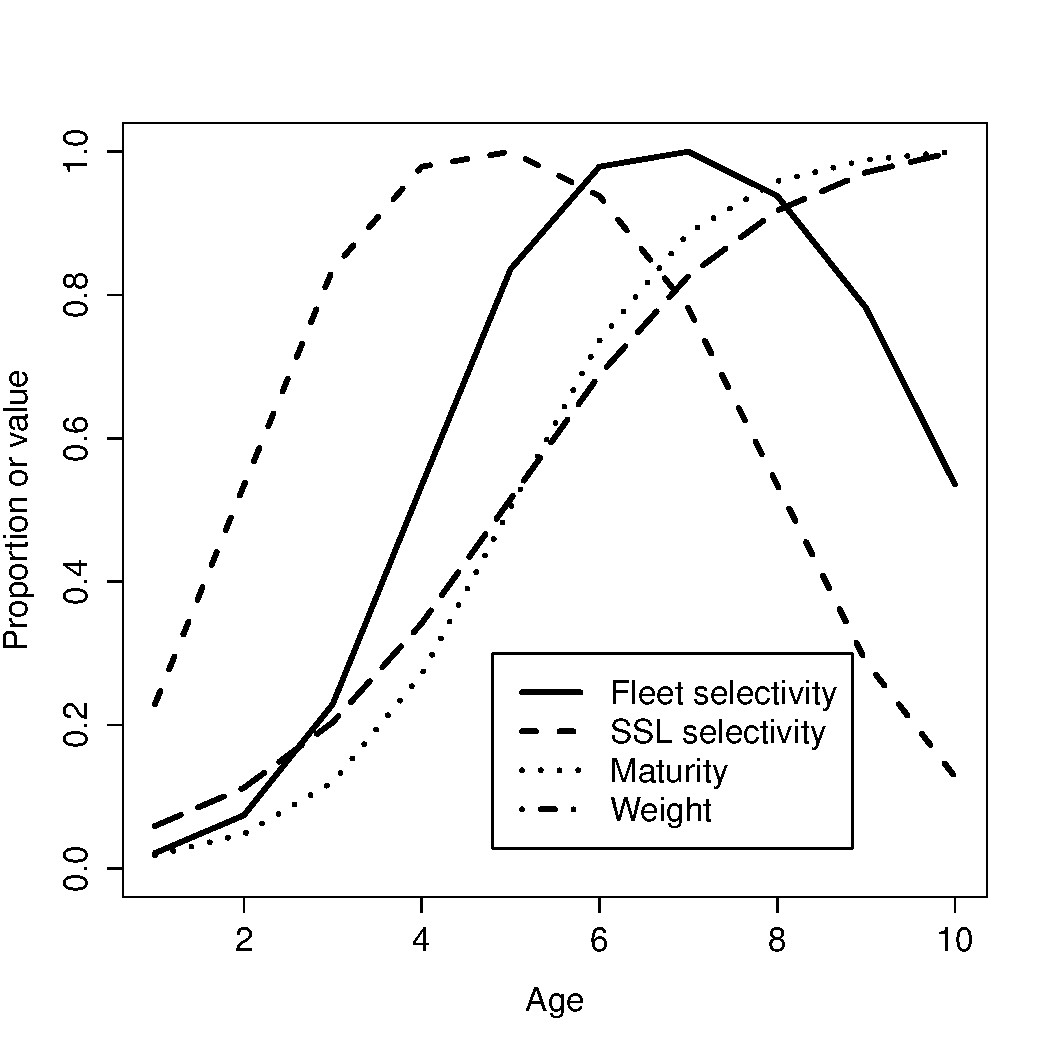
\includegraphics[width= \textwidth]{At_age_plots.pdf}
\end{center}
\caption{A depiction of fishery selectivity-at-age (`Fleet selectivity'), Steller sea lion selectivity (`SSL selectivity'), proportion of sexually
mature fish by age (`Maturity'), and weight-at-age (`Weight'; standardized to have a maximum of 1.0) used
in SSL-fisheries simulation analyses.}
\label{fig:at_age}
\end{figure}

\begin{figure}
\begin{center}
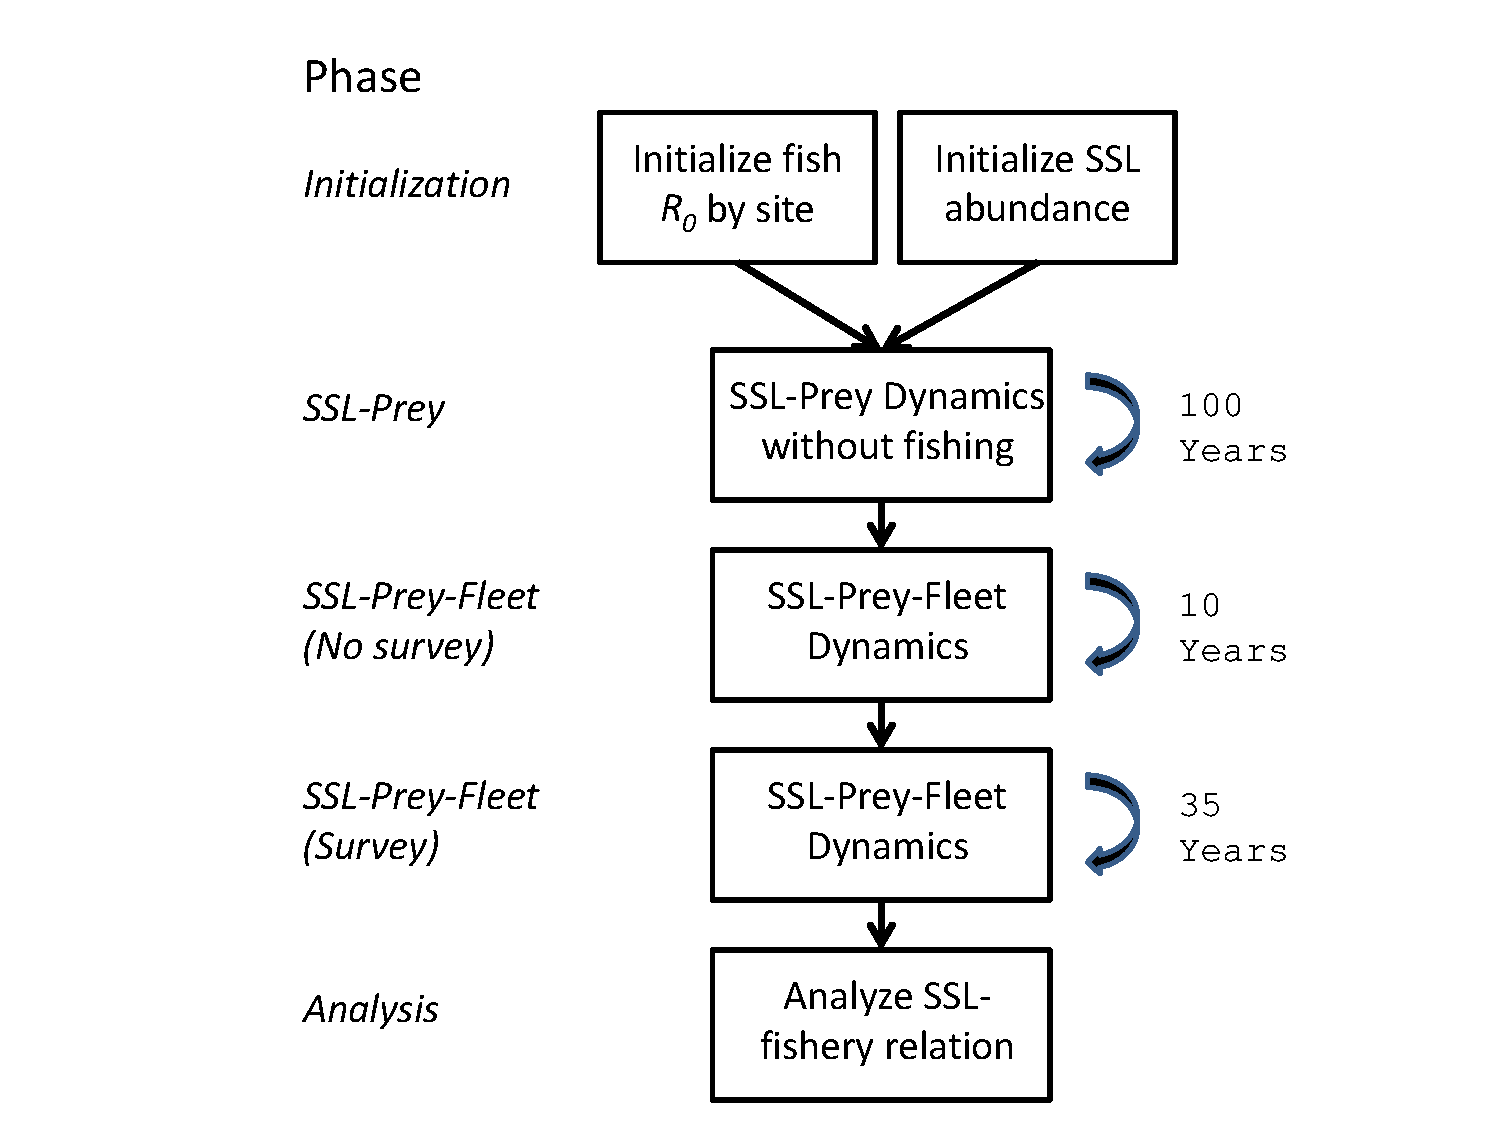
\includegraphics[width= \textwidth]{sim_diagram.pdf}
\end{center}
\caption{A depiction of the simulation structure used in analysis of Steller sea lion (SSL) and fishery
 variables.  At the beginning of each simulation, predator (SSL) and prey (fish) populations are initialized at stable age distributions. After 100 years of simulating predator-prey dynamics to equalize numbers and induce variability in age structure due to fish recruitment stochasticity, fishing is introduced.  Following 10 years of fishing with no survey, simulated aerial surveys are assumed to occur for the next 35 years (at which time catch and CPUE are also calculated).  Finally, after simulated time series are gathered, data are analyzed via generalized linear mixed models to summarize relationships between SSL and fishing variables.}
\label{fig:sim_diagram}
\end{figure}

\begin{figure}
\begin{center}
\includegraphics[width= \textwidth]{sim_trajectories.pdf}
\end{center}
\caption{Examples of simulated SSL time series resulting from calibrated models for SSL, fish, and fishery dynamics.  Five time series are displayed for each simulation scenario, with thin black lines giving total SSL numbers (in 10,000s), and thin grey lines giving scaled fish biomass.  Thick lines represent the mean trajectory over each of the 5 simulations presented.  Top panels (A and B) are representative time series for the case when SSL survival is a function of available fish biomass, while bottom panels (C and D) represent scenarios where available fish biomass affects SSL fecundity.  Left hand panels (A and C) are for cases where fishing effort is randomly allocated among island populations, while right hand panels (B and D) are for cases where fishing effort is allocated proportionally to fish abundance.}
\label{fig:sim_trajectories}
\end{figure}
\end{document}
